\documentclass[10pt,a4paper,twoside]{article}
% The following LaTeX packages must be installed on your machine: amsmath, authblk, bm, booktabs, caption, dcolumn, fancyhdr, geometry, graphicx, hyperref, latexsym, natbib

% Please make sure that spp.dat (supplied with this template) is in your working directory or path
\input{spp2024.dat}

%  Editorial staff will uncomment the next line
% \providecommand{\artnum}[0]{XX-XX}
% \renewcommand{\articlenum}[0]{SPP-\the\year-\artnum-}

\begin{document}

%--------------------------------------------------
%  Fill in the paper's title in Sentence case
%  Titles beginning with articles (A, An, The) are discouraged
%--------------------------------------------------
\title{\TitleFont Learning dynamics in a cellular automata model of classroom peer-to-peer interactions}


%--------------------------------------------------
% For TWO authors with the same affiliation please use this block
% Or Please use the other author block templates
%--------------------------------------------------
\author[*\negthickspace]{Clarence Ioakim T.~Sy}
\author[ ]{Johnrob Y.~Bantang
\lastauthorsep}
\affil[ ]{National Institute of Physics, University of the Philippines - Diliman, Philippines}
\affil[*]{\corremail{ctsy@up.edu.ph} }

%--------------------------------------------------
%  For three or more authors with the same affiliation please use this block
%--------------------------------------------------

% \author[*]{Author M.~Surname\authorsep}
% \author[ ]{Bauthor D.~Surname~Jr.\authorsep}
% \author[ ]{Cauthor D.~Surname~III\lastauthorsep}
% \affil[ ]{Department of Science, XXX University, Country}
% \affil[*]{\corremail{amsurname@university.edu} }

%--------------------------------------------------
%  For authors with different affiliations please use the following block
%--------------------------------------------------
% \author[1*]{Author M.~Surname\authorsep}
% \author[2]{Bauthor D.~Surname~Jr.\authorsep}
% \author[1,2]{Coauthor G.~Surname~III\authorsep}
% % !!! Please take note that the last author separation is \lastauthorsep instead of \authorsep
% \author[3]{Dauthor G.~Surname\lastauthorsep}
% \affil[1]{Department of Physics, DD University, Country}
% \affil[2]{Department of Science, XX University, Country}
% \affil[3]{Physics Institute, Country}
% \affil[*]{\corremail{amsurname@university.edu} }


\begin{abstract}
\noindent
%--------------------------------------------------
% Include abstract and keywords here
%--------------------------------------------------
Peer-to-peer instruction has recently become one of the popular means of classroom instruction in Physics Education. Such educational setup must involve not only physical interaction with things but also actually doing some procedural steps mentally or physically. In this study, we investigate the effects of different seating arrangements to the students' learning efficiency in the peer-to-peer mode of instruction by modelling the transfer of knowledge within the class as a probabilistic cellular automata model.  We compared the efficiency of learning between the traditional learning model and peer-to-peer learning model. We found that in square classrooms with different lengths $L \in\lbrace32,48,64,96,128\rbrace$, the inner corner seating arrangement performed the best among the peer-to-peer learning setups in terms of both the time it takes for all the students to learn ($t_{max}$) and the classroom’s learning rate ($m$). This result is different from a previous study. The difference stems from the simplifications made in this model that may not reflect real world factors. Our model uses binary values instead of continuous values as a measure of students’ aptitude, does not consider memory or unlearning and directionality or orientation bias (non-isotropic). It also does not consider the similarity effect mentioned in related literature where students learn more from peer discussion when interacting with students of a similar aptitude level regardless of how well they understand the lesson. However, despite these simplifications, we found that in smaller classrooms with slow learners, peer-to-peer learning is more efficient compared to the traditional learning model, just as previous studies has suggested.

\keywords{classroom dynamics, probabilistic cellular automata}

\end{abstract}

\maketitle
\thispagestyle{titlestyle}


%--------------------------------------------------
% the main text of your paper begins here
%--------------------------------------------------
\section{Introduction}\label{sec:intro}
Peer instruction (PI) or peer-to-peer (P2P) learning is a mode of teaching where students are given the chance to interact with their classmates to discuss ideas and questions in the classroom in addition to interactions with the teacher and traditional lectures. Although there are many ways to implement PI in the classroom \cite{knight2018peer}, one common way is for the teacher to pose a question the the class then give the class a chance to discuss their answers before re-answering the question \cite{crouch2001peer}. PI has shown to improve students' understanding for both conceptual and problem-solving skills across different subjects including calculus, physics, and life sciences \cite{crouch2001peer,smith2009peer}. Students who learned through PI also showed better conceptual understanding and similar problem solving skills compared to students who were taught traditionally \cite{lasry2008peer}. Furthermore, there are related literature that show that students' understanding of the lesson can improve after PI even if no one in the group initially knew the answer \cite{smith2009peer}. In line with this, other research has shown that students with less background knowledge that had PI opportunities in class learned as much as students with more background knowledge in the traditional set up \cite{lasry2008peer}.

\noindent A cellular automaton (CA) is a model in which agents or cells are place in a grid and can take on different states. These CA evolve over time either synchronously or asynchronously. How they evolve are dictated by rules which can either be deterministic or probabilistic in nature. In a CA, neighborhoods are defined as the set of cells that are deemed to interact with each other that may result to a change in the state of one or more cells within the same neighborhood. The neighborhood can be defined arbitrarily, but two common types in a 2D CA on a square grid are the Moore neighborhood (square) and the von Neumann neighborhood (diamond) \cite{weisstein2002cellular}. Since their introduction, CA have become computational tools that are used to model complex and dynamic systems effectively despite the relative simplicity of their rules. Probabilistic CA (PCA) are extensions of the CA model in which the rules to update the cells' states involve some randomness. Its probabilistic nature gives the model more flexibility to model physical phenomena that are also probabilistic in nature like in epidemiology and wildfire models \cite{louis2018probabilistic}. Due to the discrete nature of students' positions in the classroom and the probabilistic nature of learning, we decided that it would be apt to use a PCA to model the information propagation or learning in the classroom and to learn the dynamics of this system.


\section{Methodology}\label{sec:methods}
\textbf{Peer-to-peer (P2P) learning model.} A two-dimensional binary probabilistic cellular automata (PCA) model is used to simulate the learning of students from peer-to-peer interactions in a square classroom. The PCA rules are applied to the entire system simultaneously until the classroom is fully saturated with learned students and includes three parameters. Firstly, (1) the dimensions of the classroom ($L_1 \times L_2$) such that the size is $N=L_1 \times L_2$. In the simulations ran for this experiment, the classrooms were set to be squares with lengths $L_1 = L_2 = L \in \lbrace 32,48,64,96,128\rbrace$. This is not representative of reality and is different from the previous study \cite{roxas2010seating}. This was done because a classroom length of $L=8$ (and corresponding size of $N=64$) will not give much insight as the simulations would end too quickly and would not yield enough data points for analysis. Secondly, (2) the initial position or seating arrangement (SA) of the learned students. The SA's chosen for the simulations are based on a previous study \cite{roxas2010seating}, namely inner corner, outer corner, center, and random with the number of initial learned students being constantly $n_0 = 4$. The inner corner SA places learned students halfway between the corners of the classroom and the middle. The outer corner SA places the learned students at the classroom's corners, while the center SA places the learned students in the center of the classroom, and the random SA places the learned students randomly within the classroom. Lastly, (3) the learning coefficient matrix $\Lambda$ within a neighborhood given by:
\begin{equation}\label{eq:Lambda matrix}
  \Lambda = 
  \begin{bmatrix}
  \lambda_1 & \lambda_4 & \lambda_7\\
  \lambda_2 & \lambda_5 & \lambda_8\\
  \lambda_3 & \lambda_6 & \lambda_9\\
  \end{bmatrix} \text{.}%, \text{where } \lambda_i=\lambda \forall i \in \lbrace1...9\rbrace
\end{equation}
\noindent The learning coefficient matrix $\Lambda$ dictates the probability of the student of interest, placed at the center of the matrix, to learn from its neighbors based on the latter's relative position. In this experiment, we set $\lambda_5 = 1$. This makes it so that once the student is learned, he will stay learned in the succeeding generations. The matrix $\Lambda$ can be both isotropic (no orientation bias, all $\lambda_i$ are equal) and anisotropic (has orientation bias, not all $\lambda_i$ are equal). However, in the simulations ran for this experiment, we only considered isotropic learning with learning coefficients ($\lambda$) between 0.1 to 1.0 with increments of 0.1.  In the case of students who are at the edge of the classroom, the part of the neighborhood where there are no more students are treated as seats with unlearned students. For example, an unlearned student whose only learned neighbor is in front of them will have a $\lambda_4$ chance of learning in the next generation. In the case where an unlearned student has more than one learned student in their neighborhood, probability of learning is dictated by:
\begin{equation}
  P = 1 - \prod_{n=1}^{9}{(1-S_n\lambda_n)}
  \text{, where } S_n=
  \begin{cases}
    0 & \text{when neighbor is learned}\\
    1 & \text{when neighbor is not learned}
  \end{cases}
  \label{eq:learning probability}
\end{equation}


\noindent \textbf{Traditional learning model.}To simulate traditonal learning models where the teacher simply gives a lecture to the class, a different set of rules were applied to the 2D binary PCA model using the same parameters as in the P2P model. Instead of having a chance to learn based on a learning probability matrix $\Lambda$ and learned neighbors, each student has a chance $\lambda$ to learn from the teacher. That is, for every generation, a student has a probability $\lambda$ of transitioning from unlearned to learned. Similar to the P2P model, the simulation is considered done when the classroom is saturated with learned students.

\noindent \textbf{Time to learn ($t_{max}$) and learning rate ($m$).} From the simulations, we compared both the average number of generations it takes to saturate the classroom with learned students ($t_{max}$) and the average learning rate ($m$) across different configurations over 5 independent runs. The learning rate for each trial was obtained by fitting a power law ($y = ax^m$) to the fraction of learned students as a function of the generation number. We only considered the first $50\%$ of the data for the P2P model or the first $25\%$ of the data for the traditional model. This truncation was done so that we only fit the part of the data before the finite size effect starts to affect the simulation. %We then take the exponent as the characteristic variable or learning rate ($m$) for that independent run.

\noindent \textbf{Class size dependence.} We analyzed the dependence of the time to learn ($t_{max}$) on the class size ($N$). We took representative learning coefficients $\lambda \in \lbrace 0.1, 0.5, 0.9 \rbrace$ from the traditional model and the inner corner SA from the P2P model to see how the class size and the learning coefficient affects the time to learn. %By doing this, we can see in which situations one model can be more beneficial than the other.

\section{Results and Discussion}
The data shown in Figure \ref{fig:TTL and m vs lambda} suggests that the time to learn ($t_{max}$) does not vary significantly within the same SA when we vary the class size and learning coefficient. Among the P2P models, the inner corner seating arrangement consistently performs the best with the shortest time to learn ($t_{max}$) and the highest learning rate ($m$), while the random arrangement generally performs the worst. These findings can be attributed to the simplicity of the model which lends itself to being heavily influenced by geometric factors. Analytically, the configurations’ performance is heavily dependent on the maximum distance of any point to an initially learned student. The outer corner and center seating arrangements perform very similarly because they are geometrically one circle expanding at a constant rate. In these two configurations, the maximum distance of any unlearned student to an initially learned student is the same at $d_{\text{max, center}} = d_{\text{max, outer corner}}=\frac{L\cdot\sqrt{2}}{2}$. The inner corner seating arrangement performs the best because it minimizes this distance to $d_{\text{max, inner corner}}=\frac{L\cdot\sqrt{2}}{4}$.

\noindent The data in Figure \ref{fig:TTL and m vs lambda} also shows that the traditional learning model is generally more efficient for bigger classrooms and higher learning coefficients $\lambda$. However, this result may change if we vary the number of initially learned students with respect to the classroom size.
%figures of lambda dependence
\begin{figure}[htbp!]
  \centering
  \subfloat{\makebox[0.40\textwidth]{{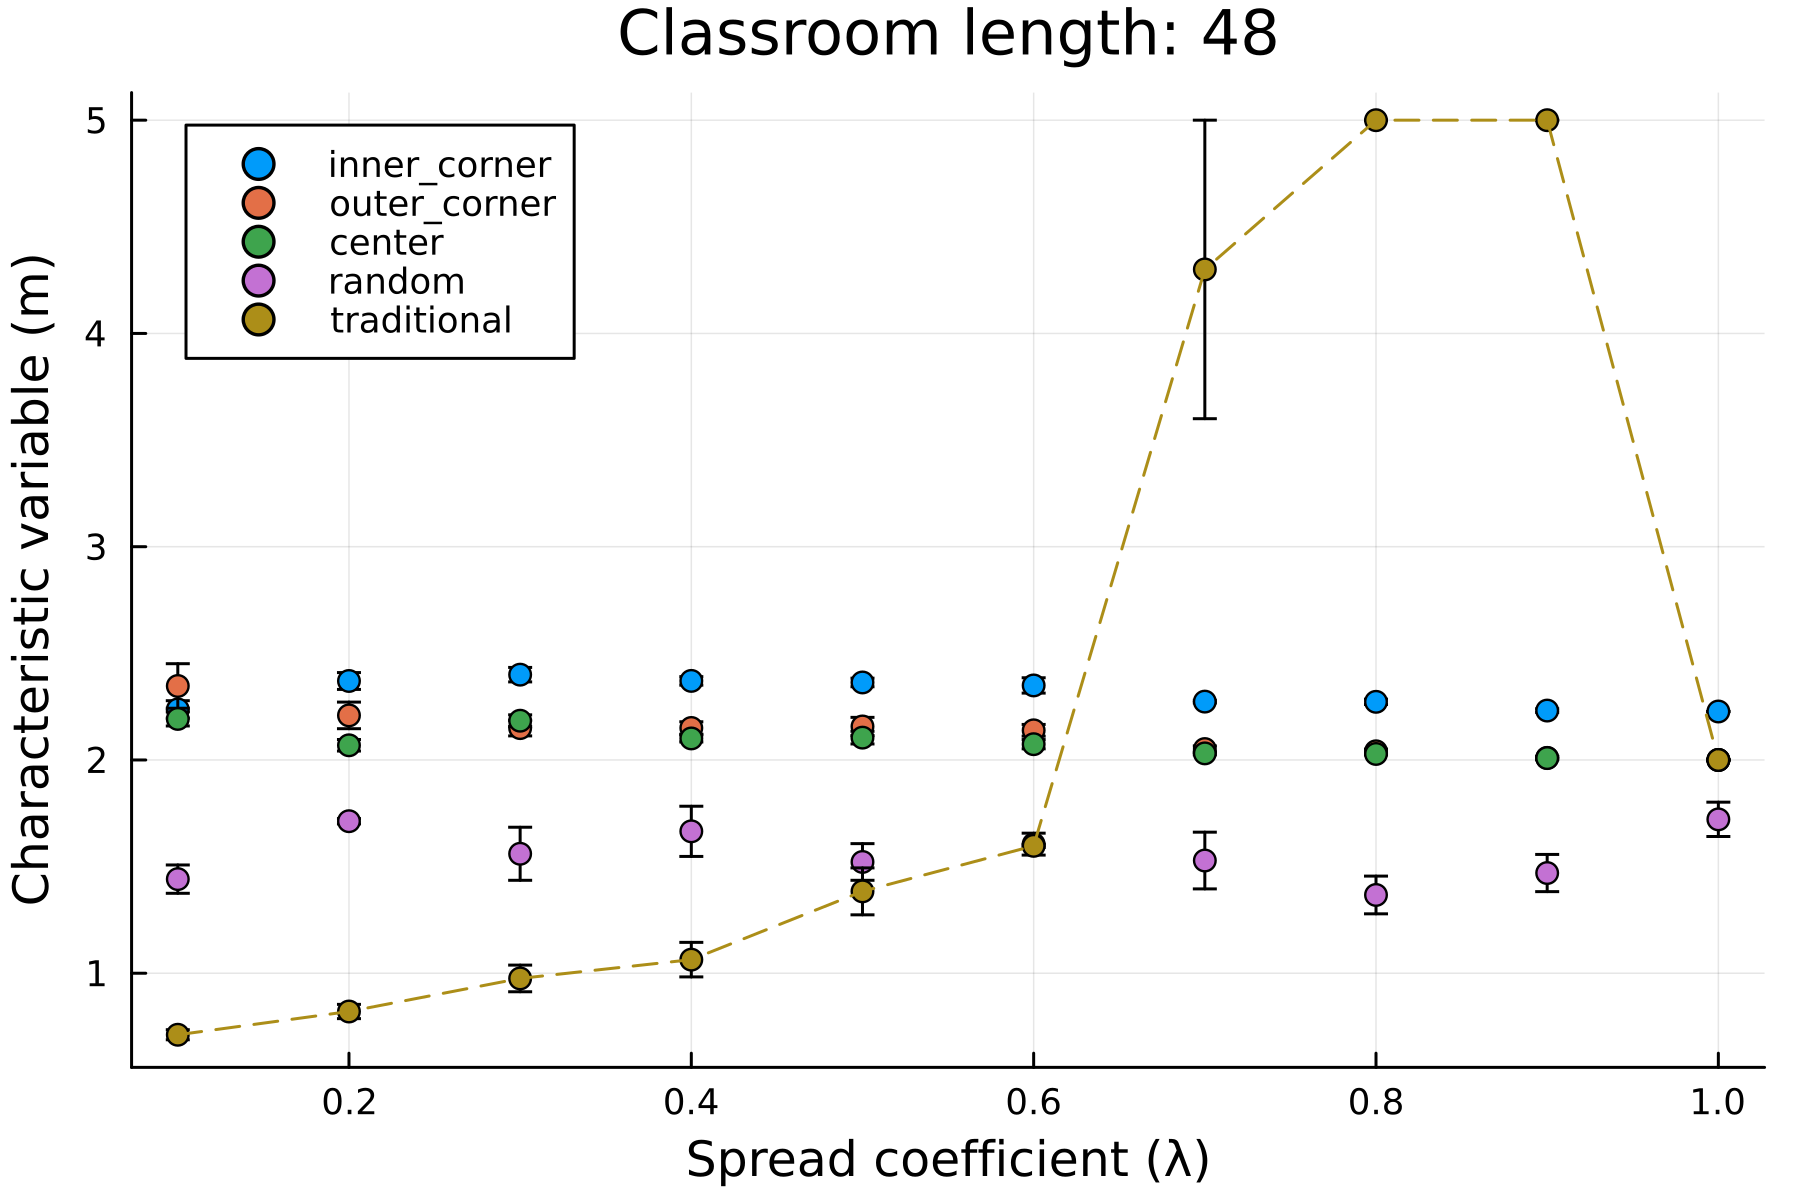
\includegraphics[width=0.40\textwidth]{figures/m-48.png}\label{fig:m-48}}}}
  \quad % or other spacing between figures
  \subfloat{\makebox[0.40\textwidth]{{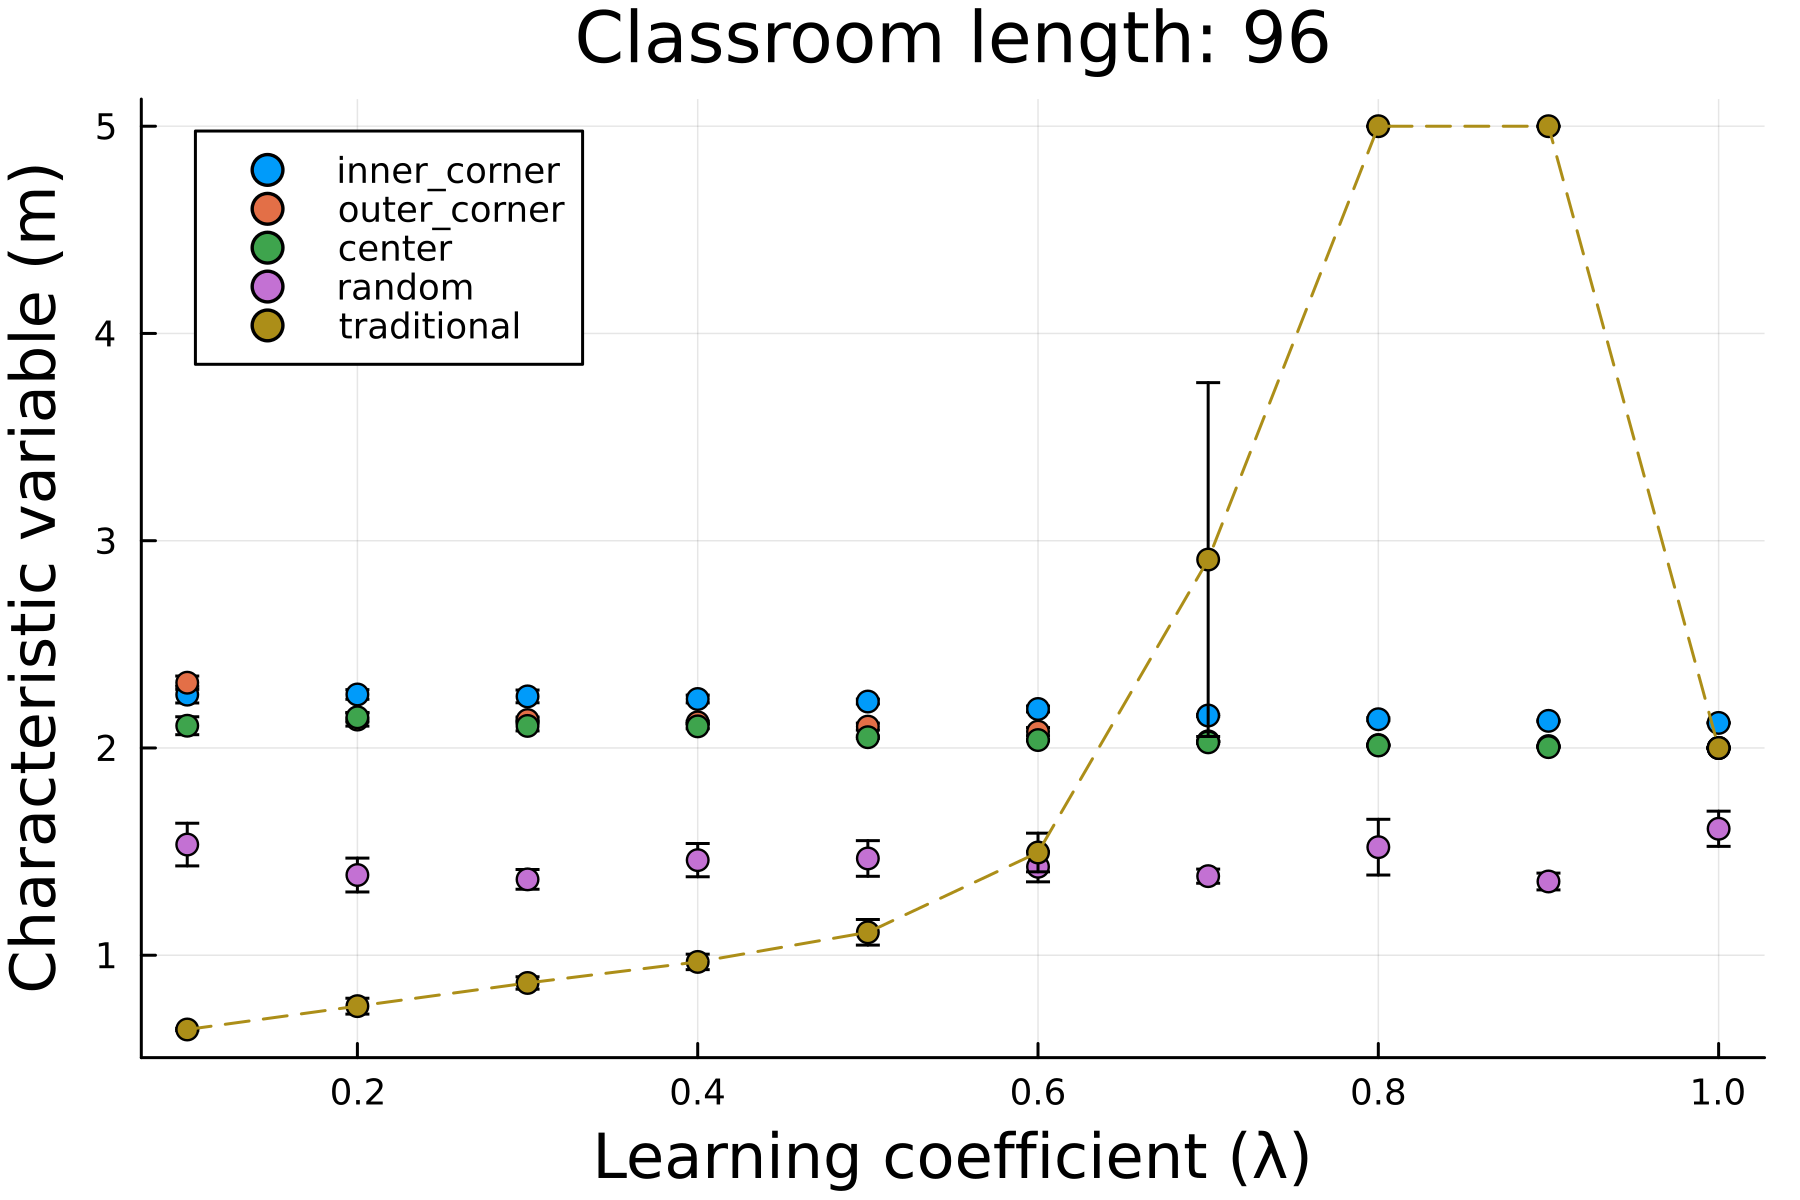
\includegraphics[width=0.40\textwidth]{figures/m-96.png}\label{fig:m-96}}}}
  \quad % or other spacing between figures

  \subfloat{\makebox[0.40\textwidth]{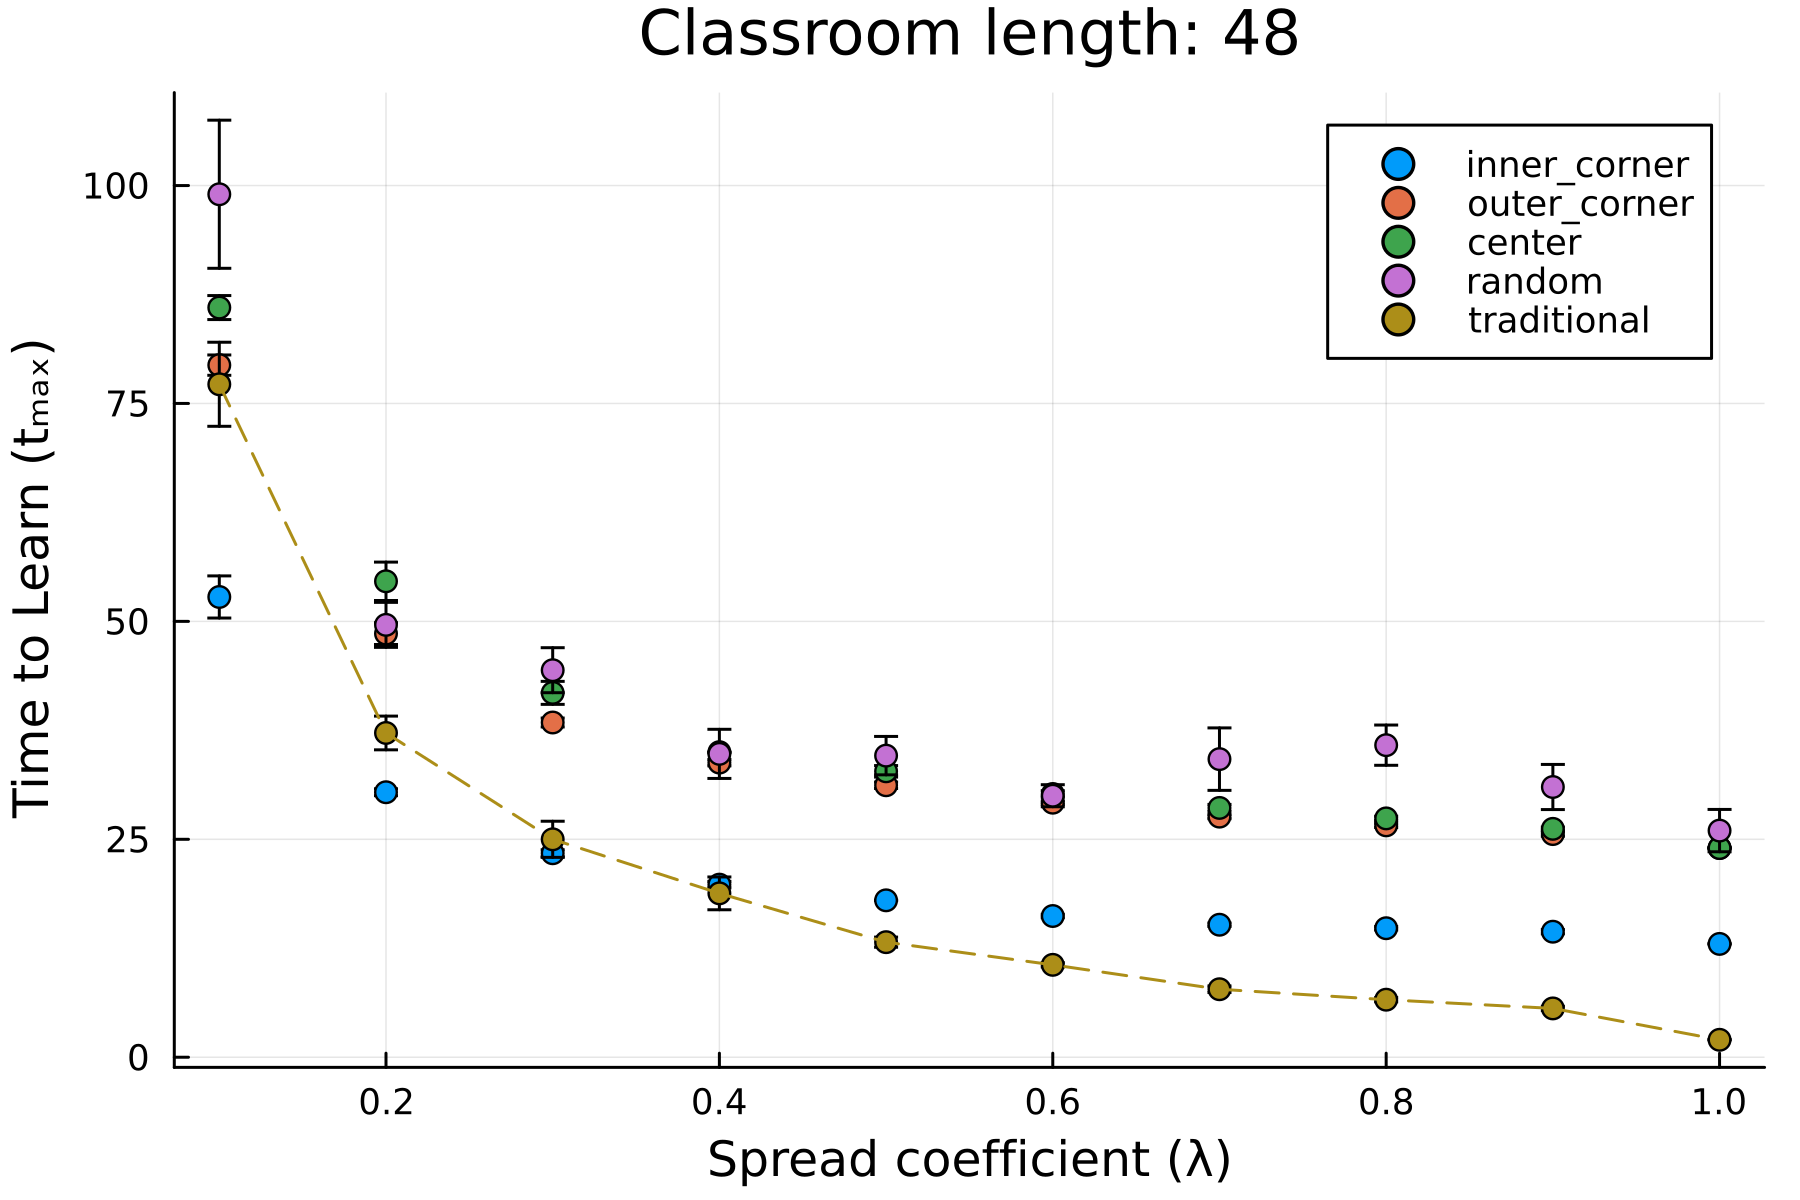
\includegraphics[width=0.40\textwidth]{figures/t-48}\label{fig:t-48}}}
  \quad % or other spacing between figures
  \subfloat{\makebox[0.40\textwidth]{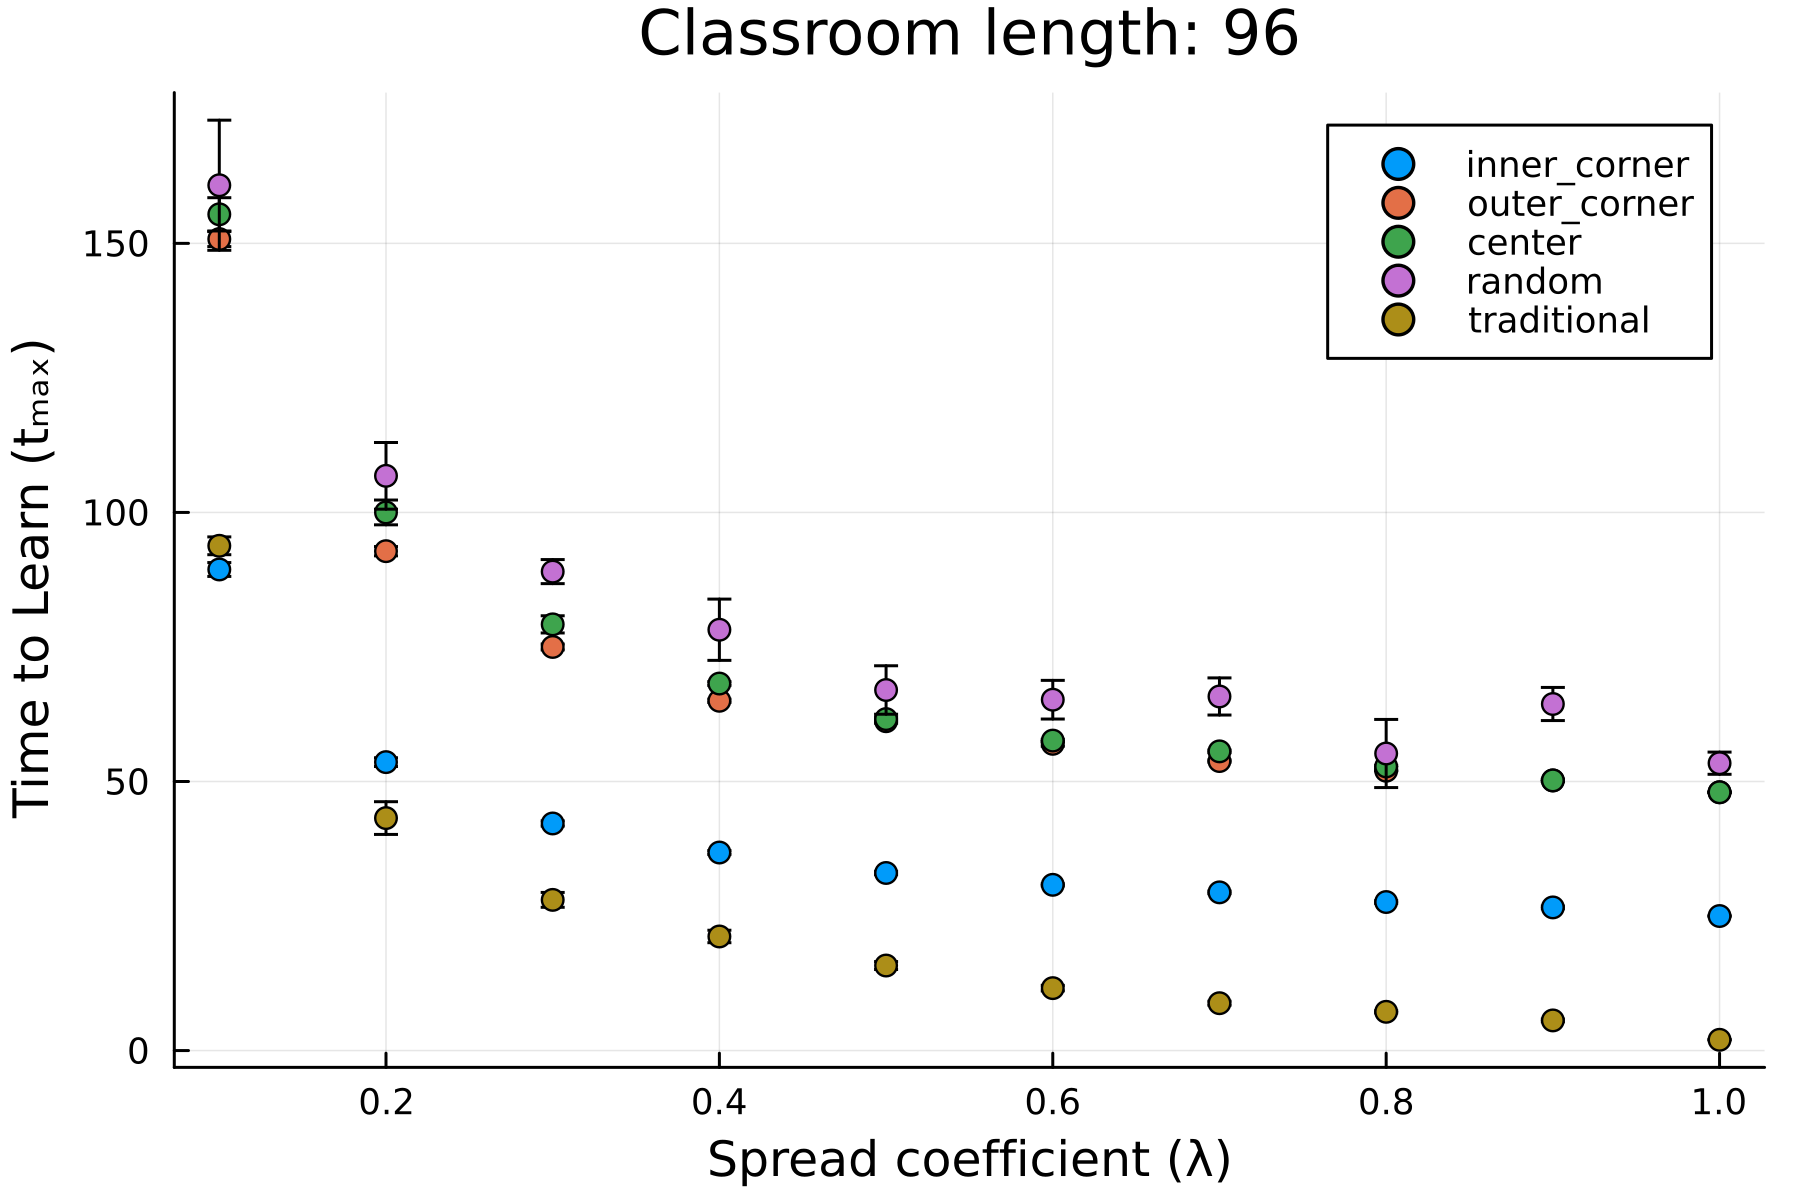
\includegraphics[width=0.40\textwidth]{figures/t-96}\label{fig:t-96}}}

  \caption{Example plots for characteristic variable ($m$) (higher is better) and time to learn ($T$) (lower is better) vs. Spread coefficient ($\lambda$) for classroom length $L \in \lbrace 48,96 \rbrace$.}
  \label{fig:TTL and m vs lambda}
\end{figure}

\noindent Our findings regarding the optimal seating arrangement for peer-to-peer learning, however, do not agree with existing studies. In a similar study \cite{roxas2010seating}, they found that the outer corner configuration performed the best in reality. The difference is expected due to the simplifications made in this study. They mentioned that there is a similarity effect that goes on in peer-to-peer learning wherein students of similar aptitude levels, regardless of their actual aptitude, learn better when seated together. The similarity effect has not yet been implemented in our system because it is not applicable to a binary system. The system being binary also introduces more granularity when compared to reality where aptitude is measured more continuously. This study also does not consider the non-isotropy or the presence of an orientation bias when it comes to the learning within each neighborhood. This study also assumes that everyone is equally receptive to learning from their peers which may not be the case, so future models should take into account the non-uniformity of individuals’ learning rates.


\noindent When we analyze the dependnce of $t_{max}$ on $N$, we see that resulting trend for both P2P and traditional models also follow the power law ($t_{max}=aN^b$). Figure \ref{fig:tmax vs N} shows that there is a point where in one model can perform better than the other. P2P learning models perform better than traditional in small classrooms with slower learners (low learning coefficient $\lambda$). This agrees with the results shown in Figure \ref{fig:TTL and m vs lambda}. It also similar to the results from previous study \cite{roxas2010seating} wherein they show that low aptitude students are the ones who benefitted the most from the P2P learning model.

%figure of TTL vs Size
\begin{figure}[h]
  \centering
  \includegraphics[width=0.9\textwidth]{figures/picture3}
  \caption{Maximum time $t_{max}$ vs class size $N$ for P2P and traditional models (lower is better). Circular symbols denote data points for the inner corner configuration for P2P learning. Rectangular denote the data points for traditional learning model. The dash lines are the power law fit in the form of $t_{max}=a \cdot N^b$ using three $\lambda$ values, $\lambda \in \lbrace 0.1, 0.5, 0.9 \rbrace$ for two cases: (1) peer-to-peer learning (inner corner configuration), and (2) traditional learning . The two major groups of power law fits are obtained based on the exponent $b$: (a) inner corner, $b = 0.432 \pm 0.019$, (b) traditional, $b=0.087\pm0.021$. The table contains the power law parameters $a$ and $b$ for each set of parameters.
  }
  \label{fig:tmax vs N}
\end{figure}

% \begin{table}[h]
%   \centering
  
%   \begin{tabular}{|c|cc|cc|}
%     \hline
%     & \multicolumn{2}{c|}{\textbf{Inner corner}}       & \multicolumn{2}{c|}{\textbf{Traditional}}        \\ \cline{2-5} 
%     & \multicolumn{1}{c|}{\textbf{$a$}} & \textbf{$b$} & \multicolumn{1}{c|}{\textbf{$a$}} & \textbf{$b$} \\ \hline
%     \textbf{$\lambda=0.1$} & \multicolumn{1}{c|}{2.4515}       & 0.3955       & \multicolumn{1}{c|}{32.4884}      & 0.1119       \\ \hline
%     \textbf{$\lambda=0.5$} & \multicolumn{1}{c|}{0.5795}       & 0.4428       & \multicolumn{1}{c|}{6.0079}       & 0.1052       \\ \hline
%     \textbf{$\lambda=0.9$} & \multicolumn{1}{c|}{0.4055}       & 0.4589       & \multicolumn{1}{c|}{3.6914}       & 0.0445       \\ \hline
%   \end{tabular}
%   \caption{Power law fit parameters $a$ and $b$ for $t_{max}$ vs $N$, where $t_{max}=a \cdot N ^ b$}
%   \label{tab:tmax vs N fit params}
% \end{table}

\noindent We see from figure \ref{fig:tmax vs N} that there are two major groups of power law fits based on their exponent or b-values: (1) those from the P2P model (inner corner SA) with $\bar{b} = 0.432 \pm 0.019$, (2) those from the traditional model with $\bar{b}=0.087\pm0.021$. From this, we can say that the traditional learning model is more scalable or that it is less size dependent compared to the P2P model. Numerically, this is explained by the lower b-values of the traditional models vs the P2P models. 

\noindent We found that b-values generally increase as the learning coefficient $\lambda$ increases as shown in Figure \ref{fig:tmax vs N}. This suggests that in classrooms with higher aptitude students are more affected by the class size than classrooms with lower aptitude students.


\section{Conclusions}
Our model was able to identify when one mode of teaching is more advantageous than the other. Classrooms with slow learners benefit the most from peer-to-peer learning methods and classrooms with fast learners are likely better off with traditional learning methods. This is in line with the existing research on this topic. However, due to the simplifications made in our model, our results in comparing between different SA's in the peer-to-peer learning model were heavily influence by geometric biases and only approximates reality. 
\section*{Acknowledgments}
Here are the acknowledgments. Note the asterisk \textbackslash{\ttfamily section*}\{{\ttfamily Acknowledgments}\} that signifies that this section is unnumbered.

% Please use the style file spp-bst.bst. If you wish to use BibTeX, kindly use us the filename bibfile.bib for your bib file.
\bibliographystyle{spp-bst}
\bibliography{bibfile}

\end{document}